\documentclass[a4paper]{article}

\usepackage[pdfauthor=Zhang~Yichi,pdftitle=Predicting~pH~from~SERS~Data]{hyperref}
\usepackage{amsmath,amsfonts,amsthm}
\usepackage{longtable}
\usepackage{graphicx}
\usepackage{natbib}
\usepackage{enumerate}
\usepackage[margin=3cm]{geometry}
\usepackage{listings}
\usepackage{xcolor}
\pagestyle{plain}
\bibliographystyle{unsrt}
\lstset{
		numbers=left,
		numberstyle=\scriptsize,
		%frame=single,
		fontadjust=false,
		flexiblecolumns=true,
		basicstyle=\ttfamily\small,
		commentstyle=\color{bladck},
		keywordstyle=\color{blue!70},
		rulesepcolor=\color{red!20!green!20!blue!20},
		escapeinside=``,
		showstringspaces=false,
		breaklines
		}

\newcommand{\ud}{\mathrm{d}}
\newcommand{\bfv}{\mathbf{v}}
\newcommand{\bfw}{\mathbf{w}}
\newcommand{\bfx}{\mathbf{x}}
		
\begin{document}
\title{\textbf{Predicting pH from SERS Data}}
\author{Zhang Yichi}
\date{August 2014}
\maketitle

\section{Introduction}
Blood tests are often used in health care to determine physiological and biochemical states of patients. But using the traditional way, we need to draw blood from patients first and it does take some time to have some tests on it. 

Recently, the chemists found that gold nanoshells can be used as intracellular sensors based on surface-enhanced Raman scattering (SERS) and these materials exhibit low toxicity to the cells of interest. This is a very good property since we can just put the nanoshell into the blood vessel of patients and measure redox potential or pH values of patients' blood instantly.

So when given the spectrum, the problem is how to predict the pH value. We have tried four regression methods, that is principal component regression (PCR), partial least squared regression (PLSR), lasso regression and kernel regression, on the data.

\section{Data}
There are 120 samples in the dataset by 2 chips. For each chip, there are 5 replications for 12 pH values, that is 60 samples. The spectrum is a 1044 dimension vector for each sample, and each dimension represents a Raman intensity for a Raman shift.

There are 2 datasets we have got for experiments. The first dataset we used was produced with the order that pH value is increasing. We have found in the dataset that the intensity is lower and lower when the pH value is greater than 7 as shown in Figure \ref{pic1}.

\begin{figure}[h]
  \centering
  % Requires \usepackage{graphicx}
  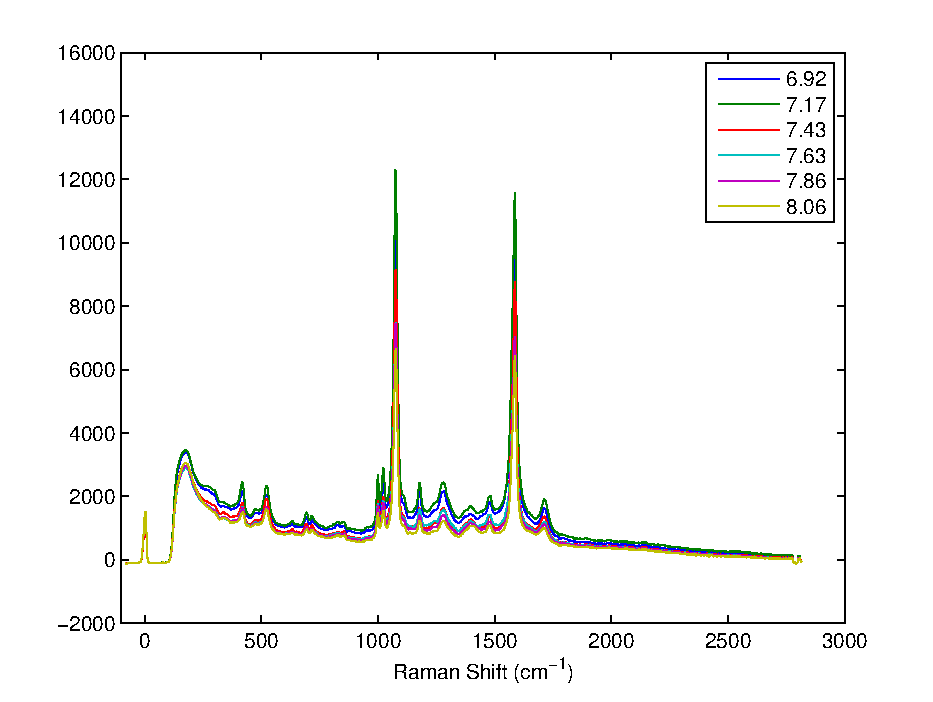
\includegraphics[width=.6\textwidth]{images/compare.pdf}\\
  \caption{The mean spectrum for different pH values in the first dataset}\label{pic1}
\end{figure}

However, the chemists have told us that the intensity is lower and lower maybe due to the systematic loss of nanoparticles through time.

Thus, we got a another set of data with pH values measured in a randomized order produced by chemists. The experiments and analyses below are based on the randomized dataset.
\subsection{Raw Data}
As for the raw data, we plot the 5 replications in one plot for each pH values as shown in Figure \ref{pic2}.
\begin{figure}[h]
\centering
\begin{tabular}{ccc}
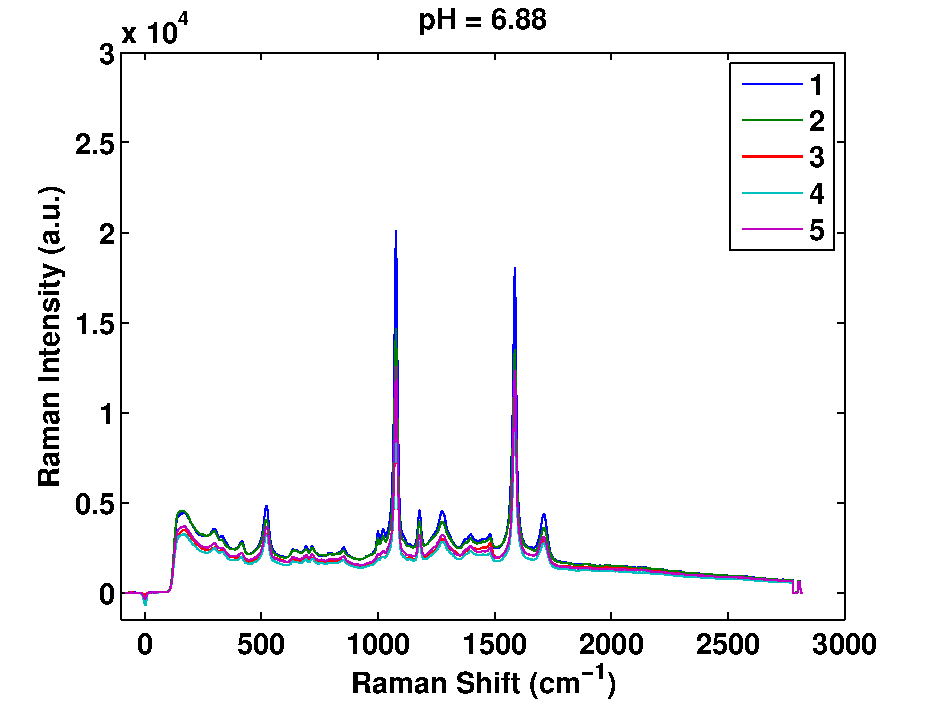
\includegraphics[width=.33\textwidth]{images/1.pdf}  & 
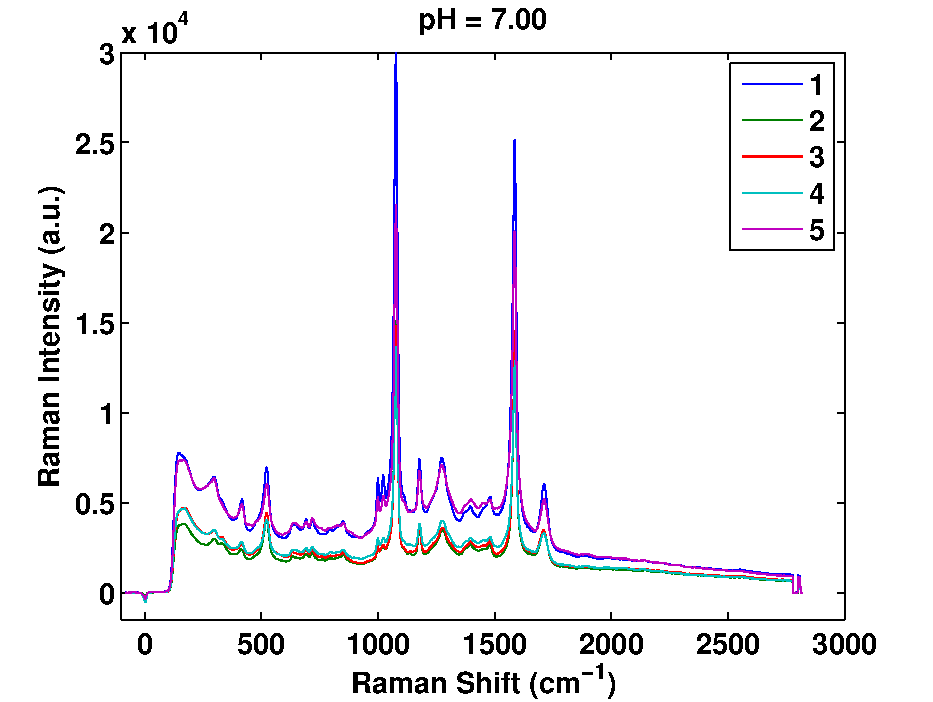
\includegraphics[width=.33\textwidth]{images/2.pdf}  &
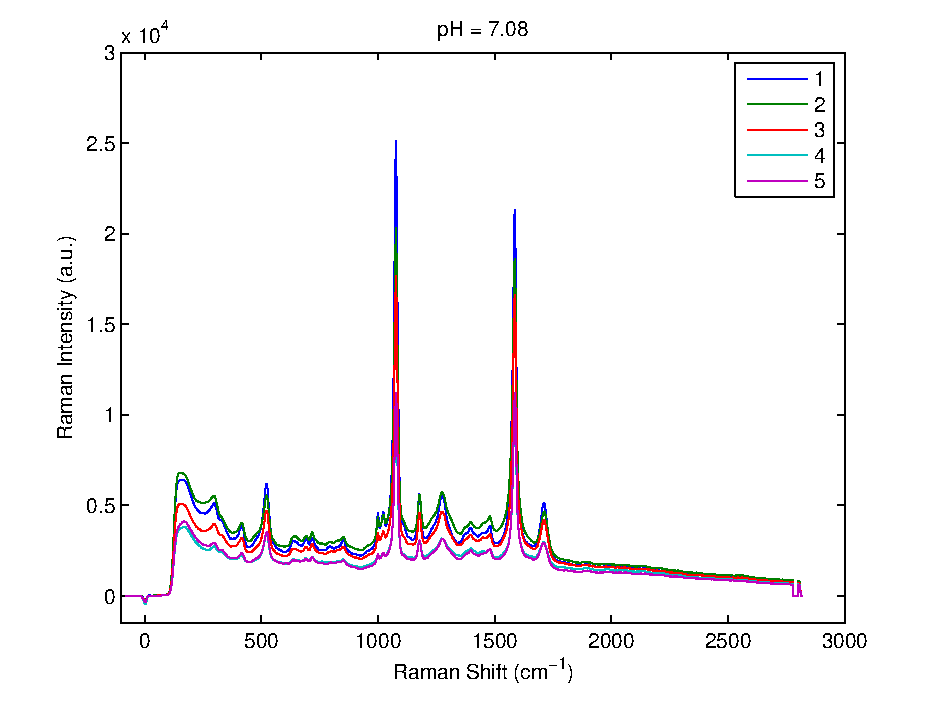
\includegraphics[width=.33\textwidth]{images/3.pdf}  \\ 
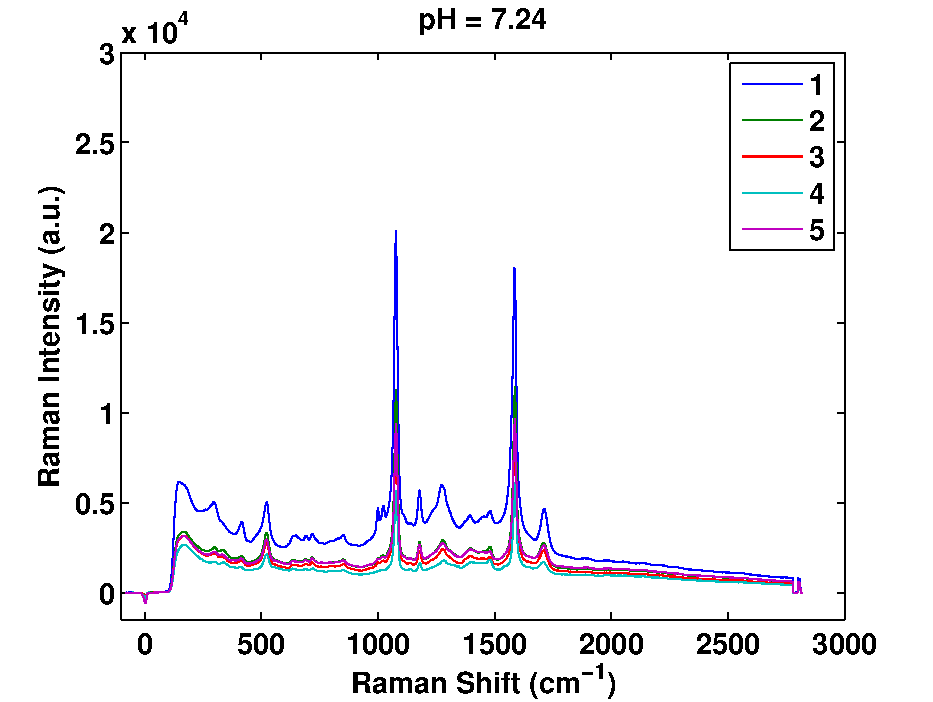
\includegraphics[width=.33\textwidth]{images/4.pdf}  &
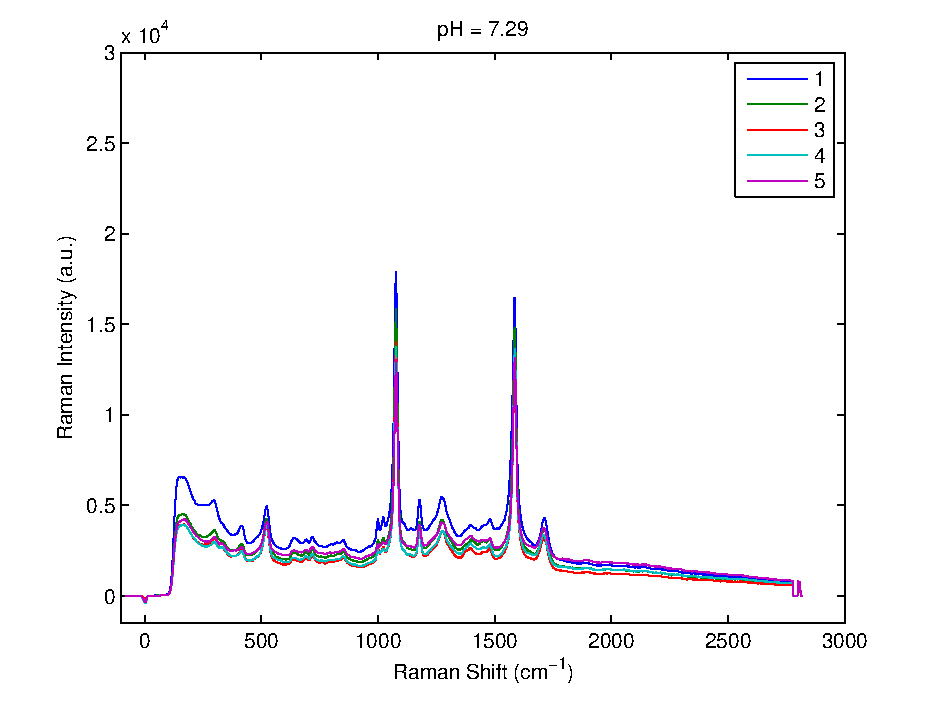
\includegraphics[width=.33\textwidth]{images/5.pdf}  & 
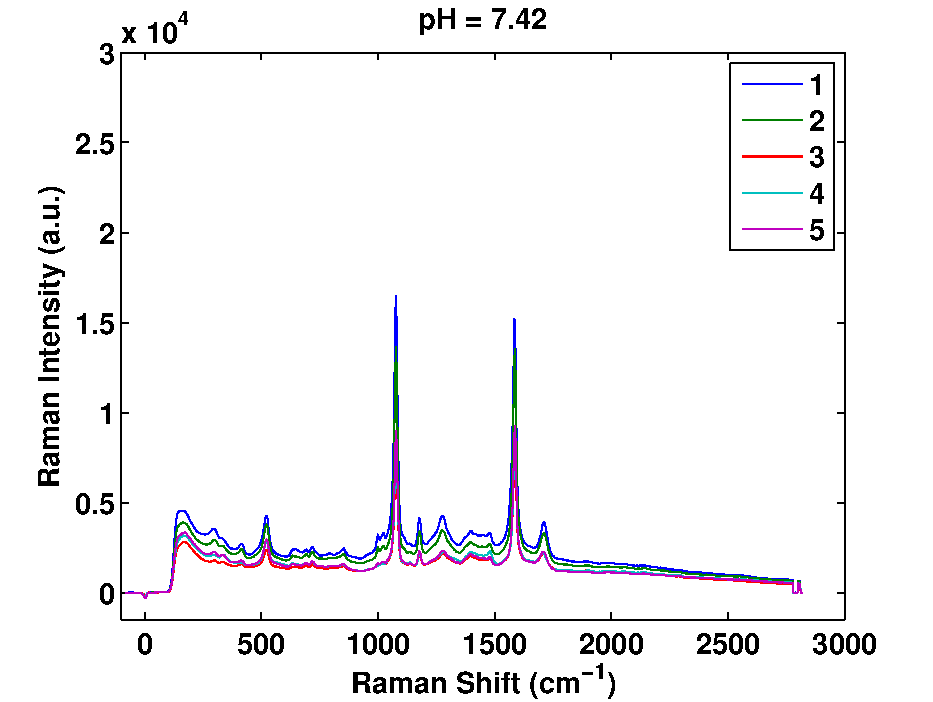
\includegraphics[width=.33\textwidth]{images/6.pdf}  \\
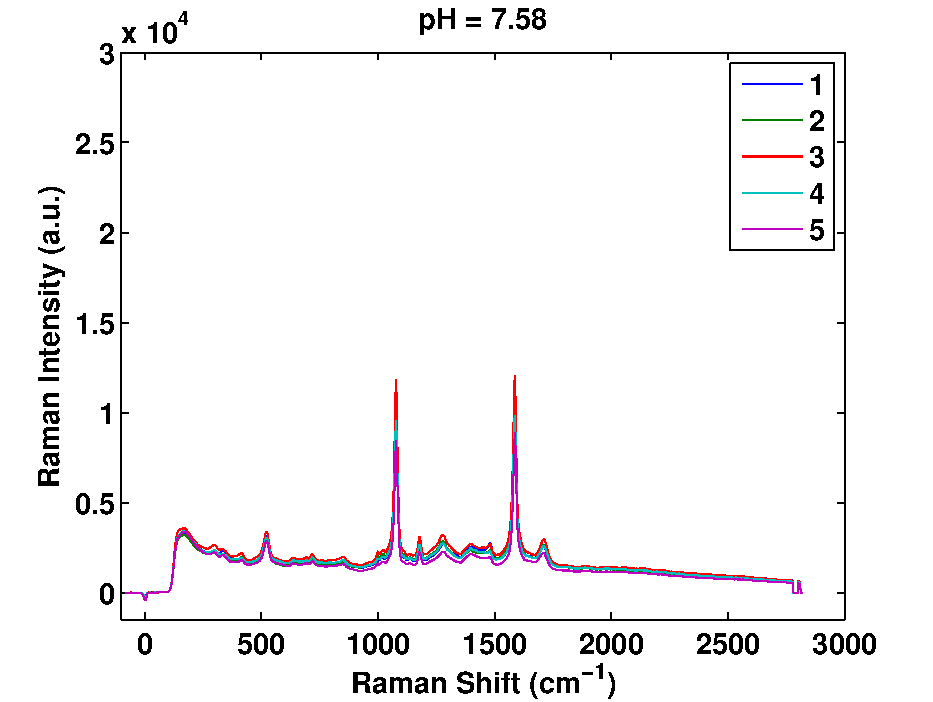
\includegraphics[width=.33\textwidth]{images/7.pdf}  & 
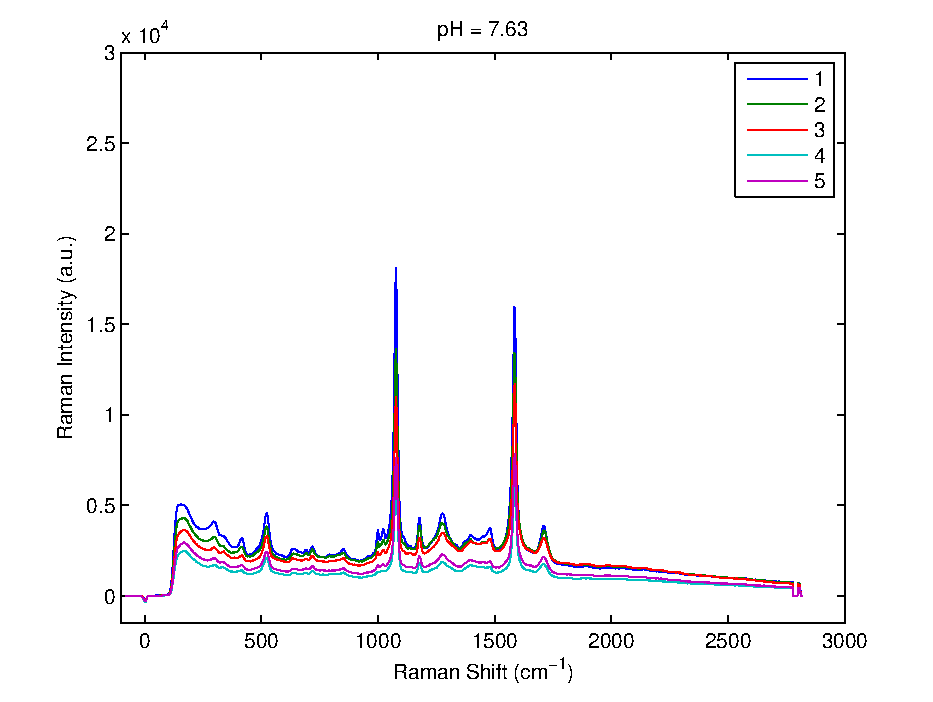
\includegraphics[width=.33\textwidth]{images/8.pdf}  &
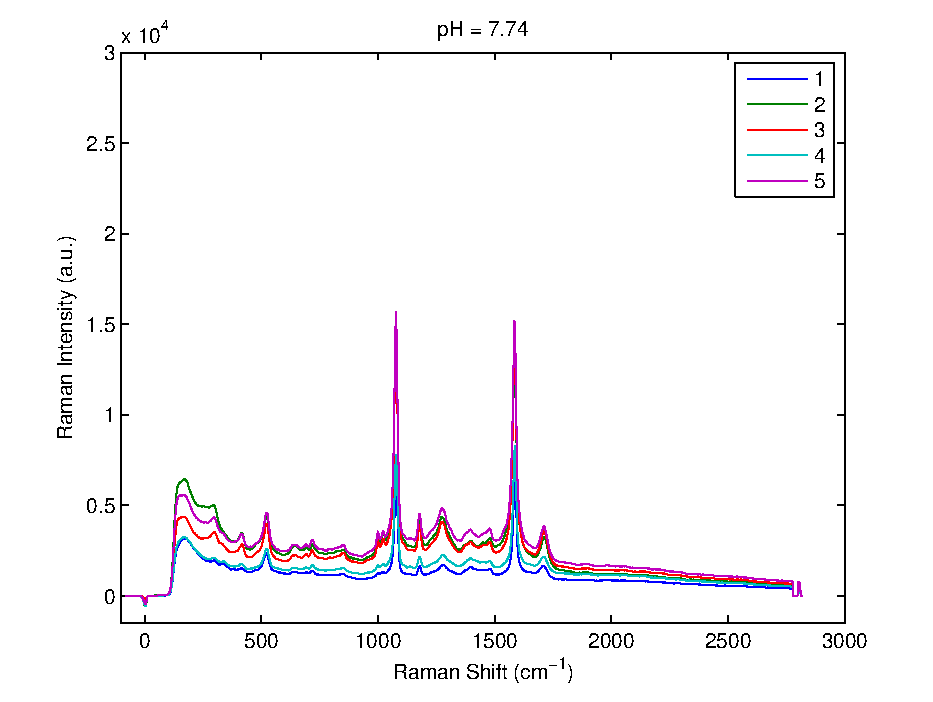
\includegraphics[width=.33\textwidth]{images/9.pdf}  \\ 
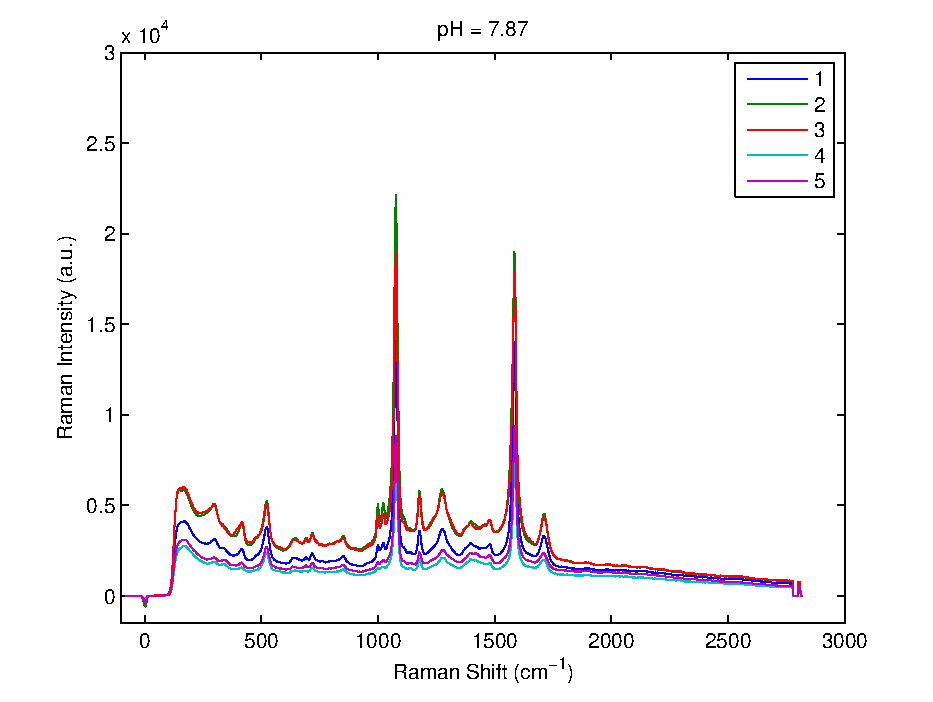
\includegraphics[width=.33\textwidth]{images/10.pdf} &
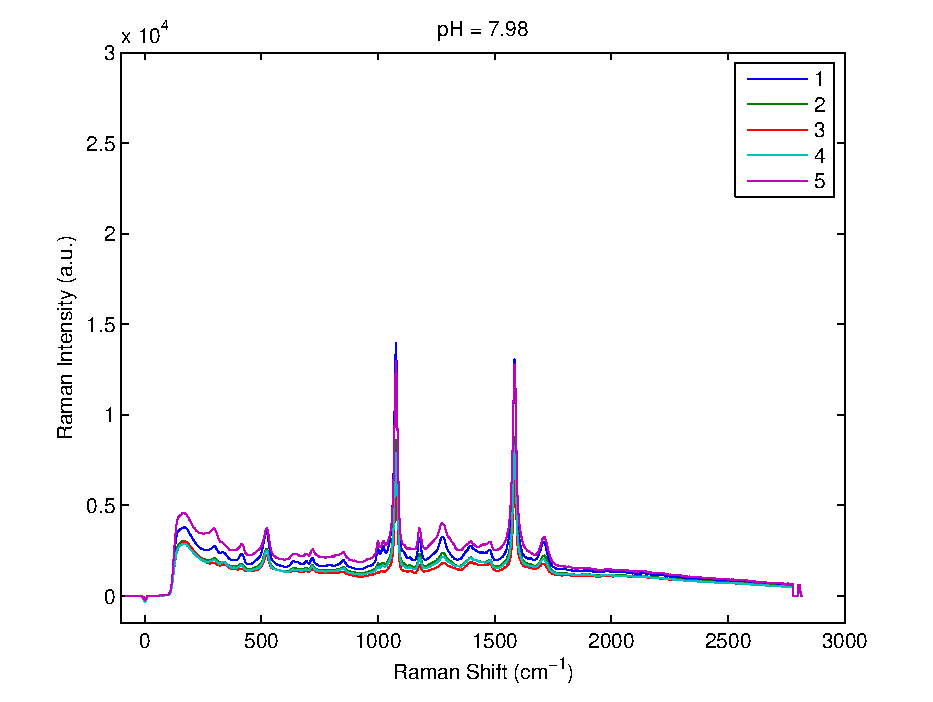
\includegraphics[width=.33\textwidth]{images/11.pdf} & 
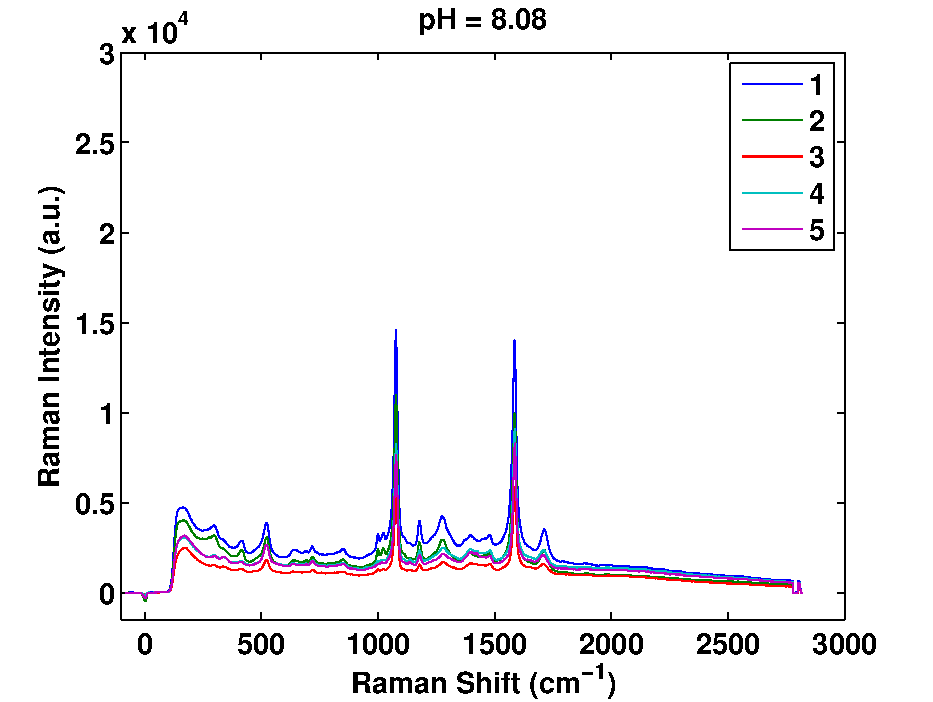
\includegraphics[width=.33\textwidth]{images/12.pdf} \\
\end{tabular}
\caption{Plots for each pH values of raw data}\label{pic2}
\end{figure}

We can find that when the pH value is increasing, not like in the previous dataset, the peak isn't lower and lower as the pH value is increasing all the time.

Meanwhile, we can find that for some pH values, the curves look dramatically different for the same pH value due to the systematic loss of nanoparticles. Suggested by chemists, normalization is a good way to avoid such variation. The method we used is normalizing the total area under the curve.
\subsection{Normalization}
As mentioned in previous section, I have normalized the total area under the curve for every spectrum as shown in Figure \ref{pic3}.
\begin{figure}[h]
\centering
\begin{tabular}{ccc}
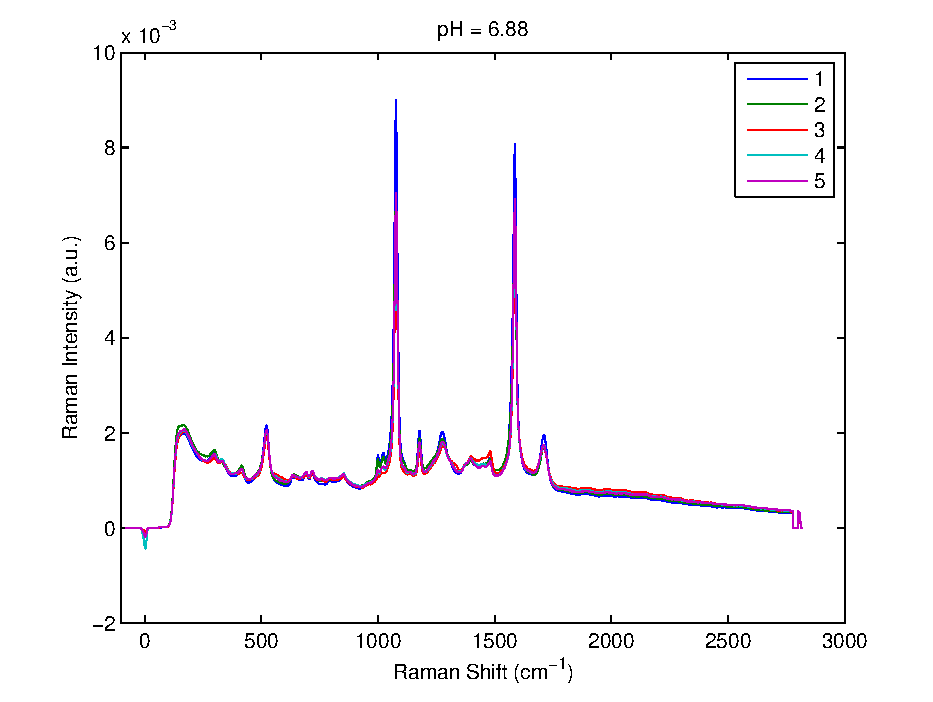
\includegraphics[width=.33\textwidth]{images/n1.pdf}  & 
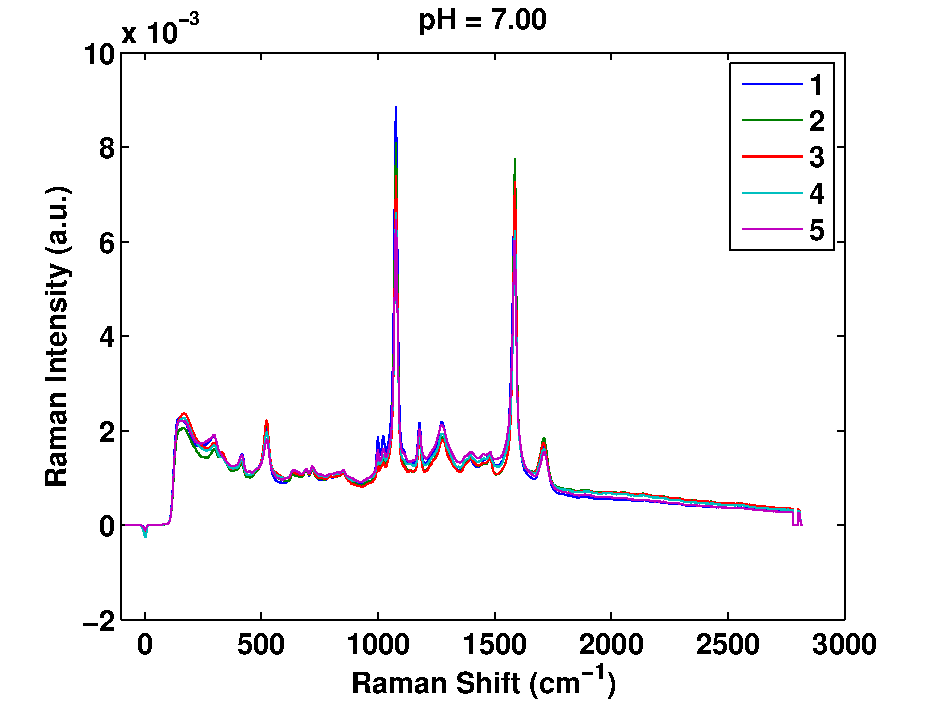
\includegraphics[width=.33\textwidth]{images/n2.pdf}  &
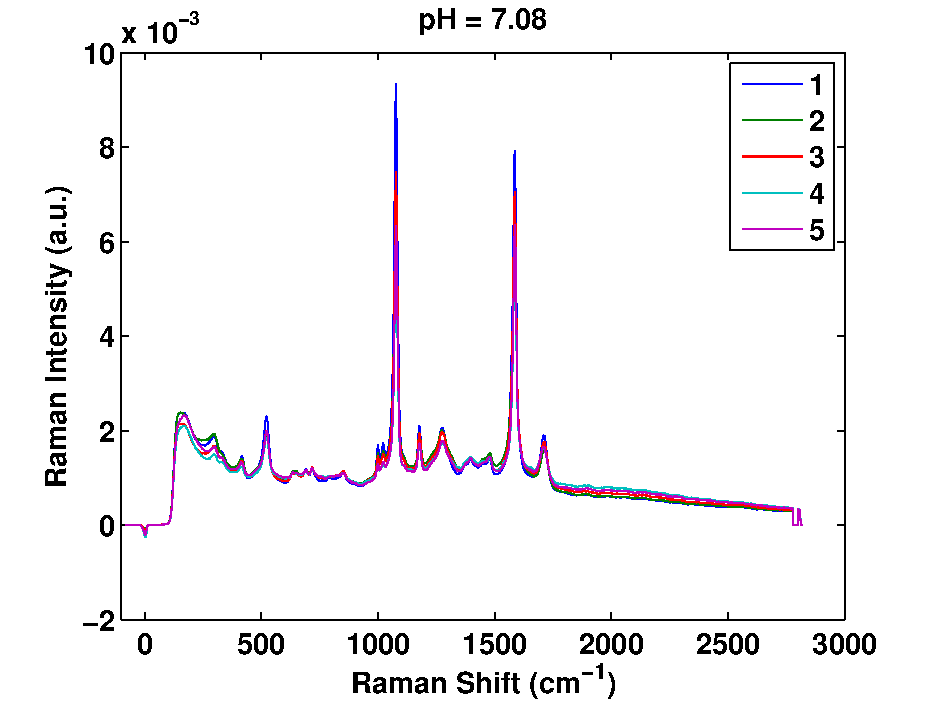
\includegraphics[width=.33\textwidth]{images/n3.pdf}  \\ 
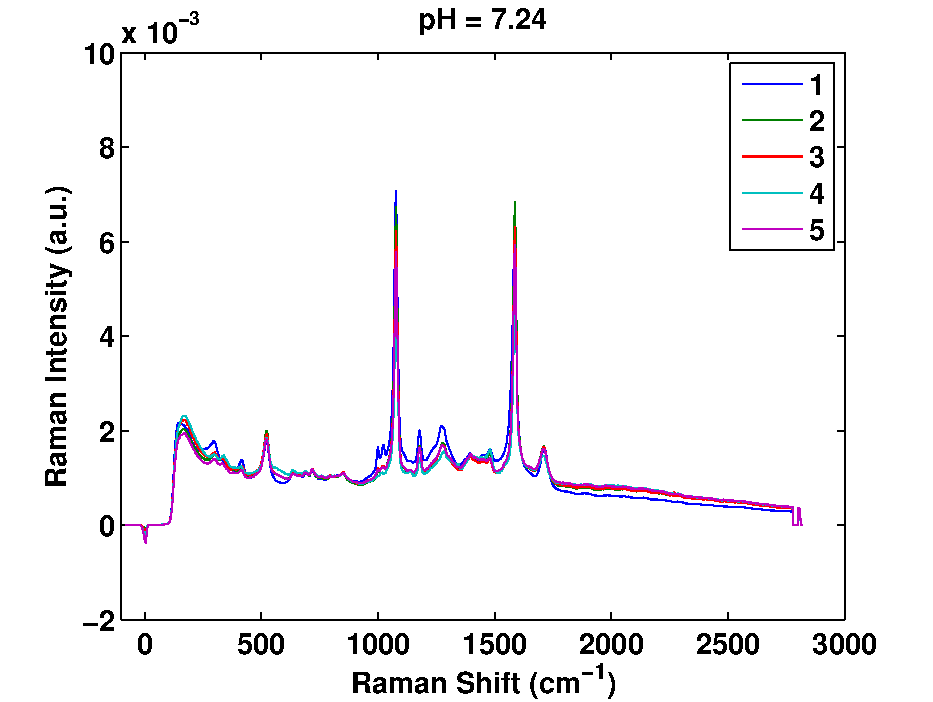
\includegraphics[width=.33\textwidth]{images/n4.pdf}  &
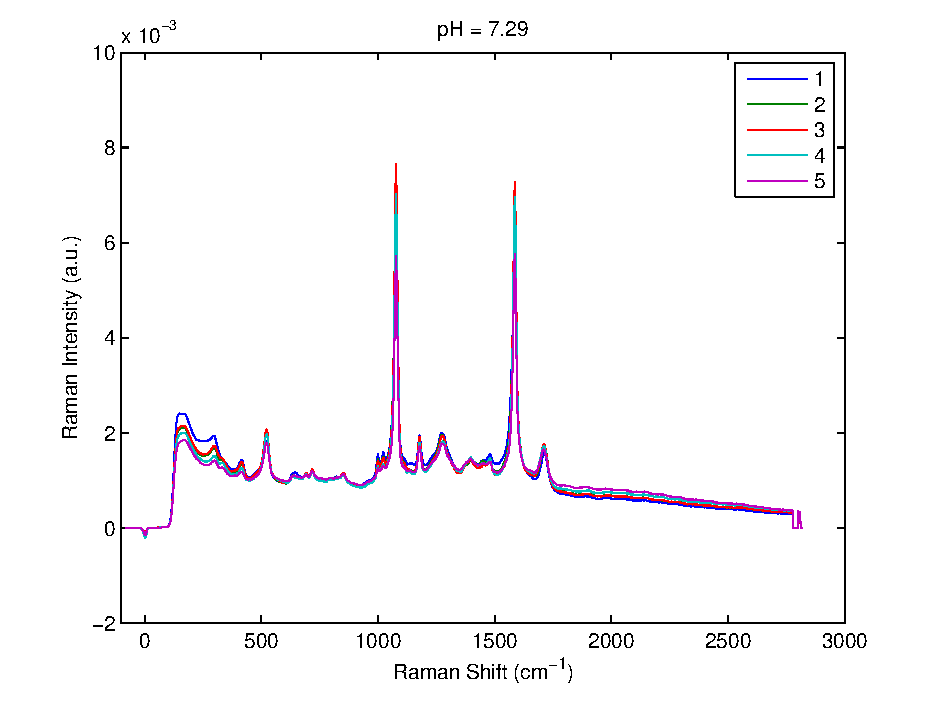
\includegraphics[width=.33\textwidth]{images/n5.pdf}  & 
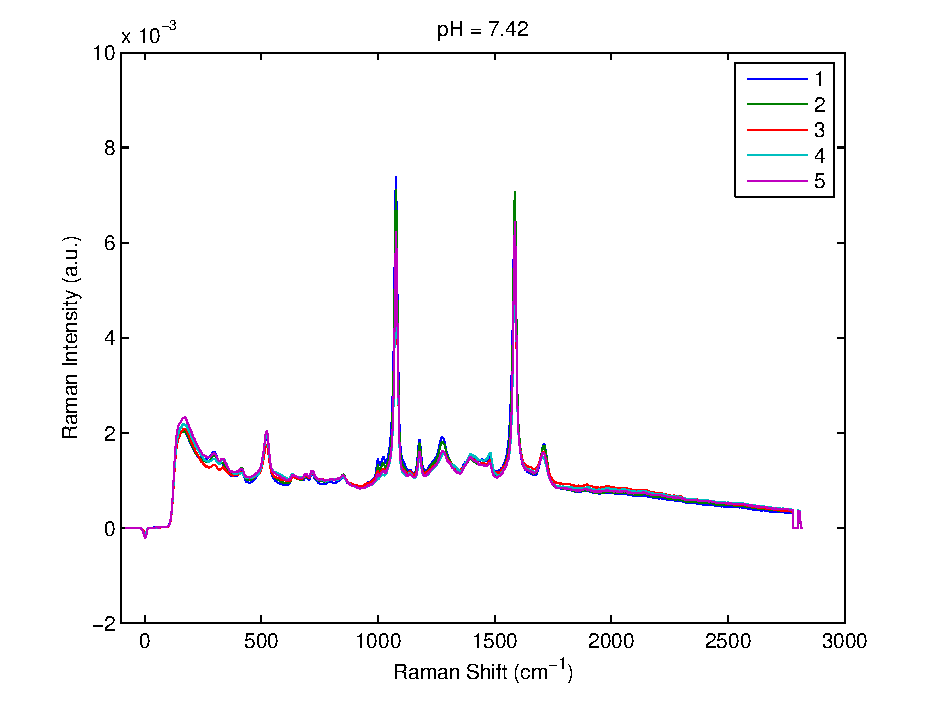
\includegraphics[width=.33\textwidth]{images/n6.pdf}  \\
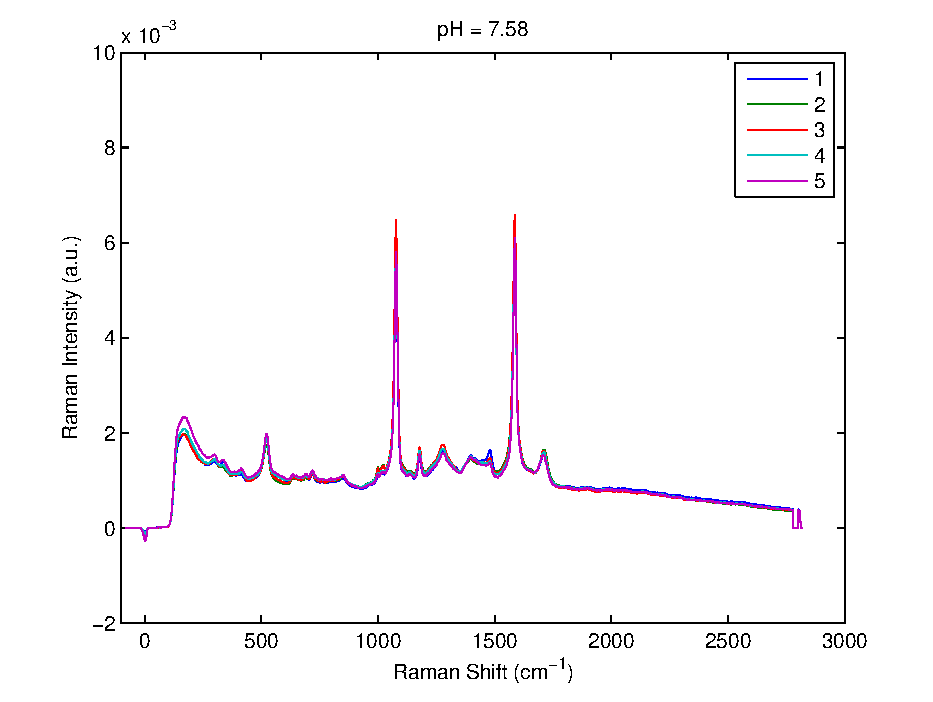
\includegraphics[width=.33\textwidth]{images/n7.pdf}  & 
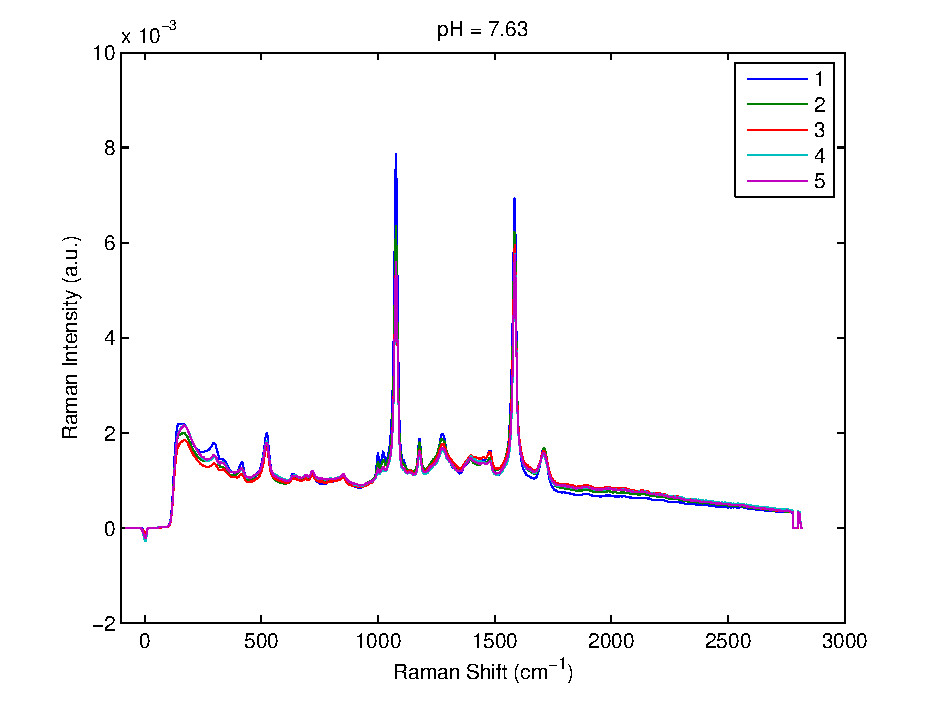
\includegraphics[width=.33\textwidth]{images/n8.pdf}  &
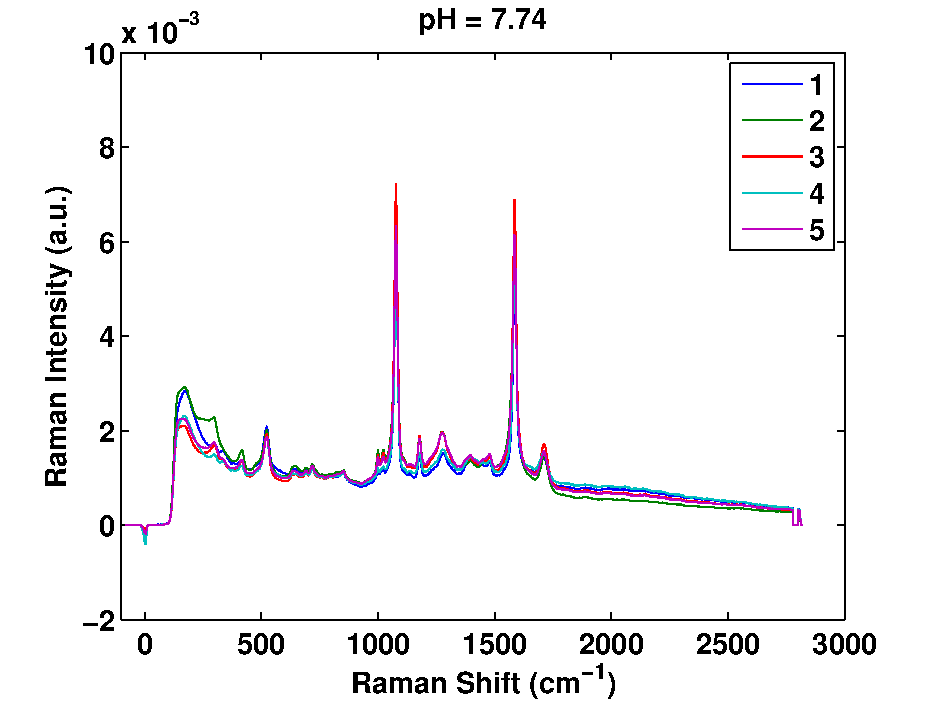
\includegraphics[width=.33\textwidth]{images/n9.pdf}  \\ 
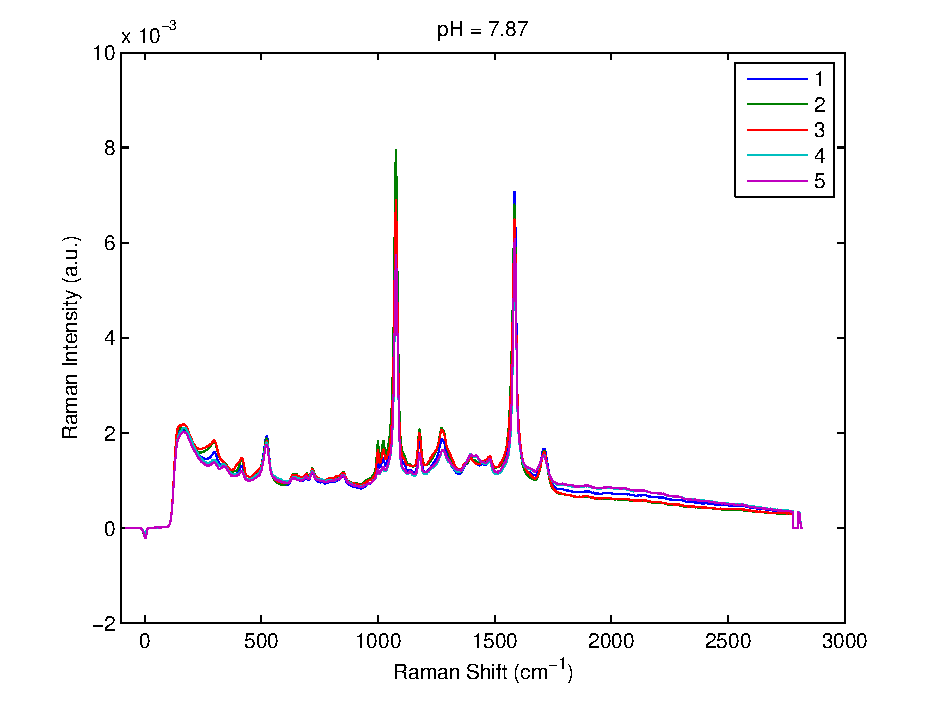
\includegraphics[width=.33\textwidth]{images/n10.pdf} &
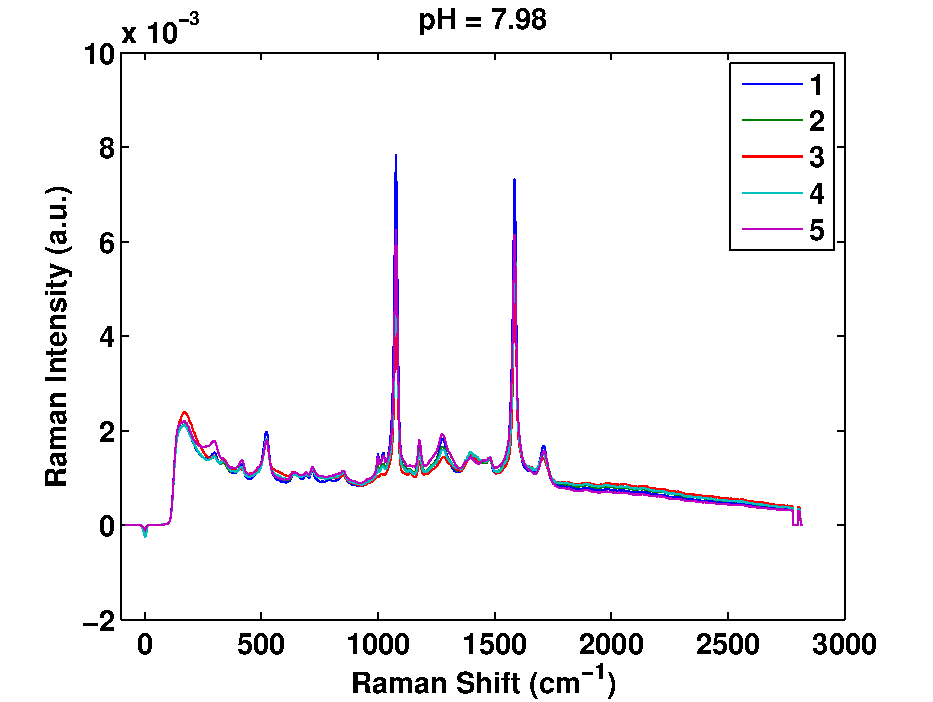
\includegraphics[width=.33\textwidth]{images/n11.pdf} & 
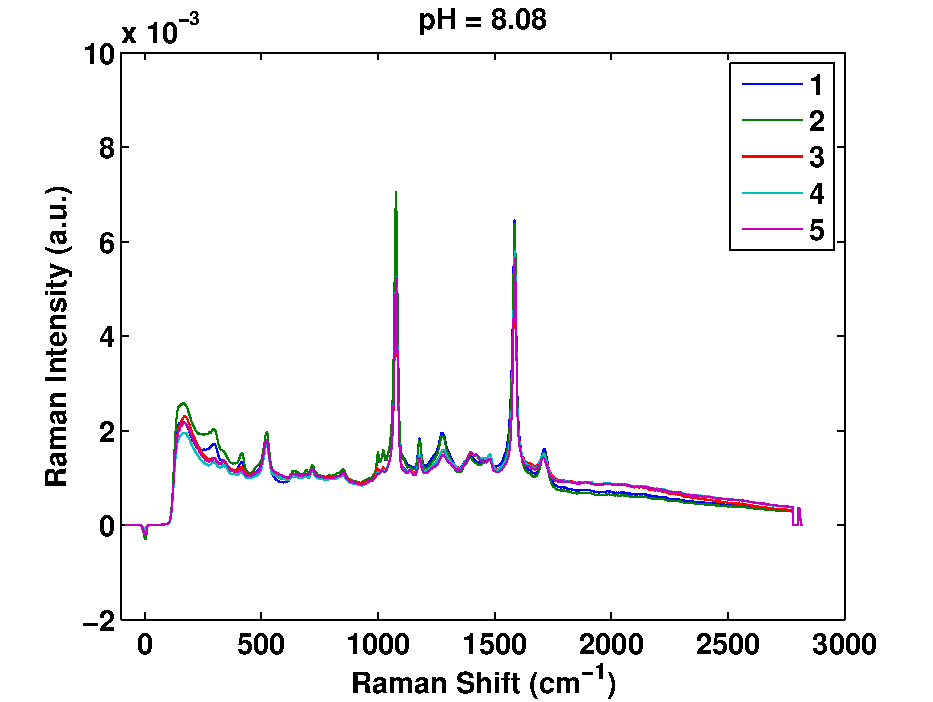
\includegraphics[width=.33\textwidth]{images/n12.pdf} \\
\end{tabular}
\caption{Plots for each pH values of data after normalization}\label{pic3}
\end{figure}

As we can see from the figure that the normalization does eliminate the differences among samples of the same pH value.
\section{Methods}
There are only 60 samples. Since the number of sample is very small, we'll use cross validation to judge which method is better.

For cross validation, we divide samples into 5 folds. For each fold, there are not two samples with the same pH value. Every time, we use 4 folds for training and 1 fold for testing, and use standardized mean squared error (SMSE)%, mean absolute error (MAE) and coefficient of determination ($R^2$) for evaluation. 
\begin{equation}
\mathrm{SMSE}=\frac{\displaystyle \sum_{i=1}^n (y_i-\hat{y_i})^2}{\displaystyle \sum_{i=1}^n (y_i-\overline{y})^2}.
\end{equation}
%\begin{equation}
%\mathrm{MAE}=\frac{1}{n} \sum_{i=1}^n |y_i - \hat{y_i}|
%\end{equation}
%\begin{equation}
%R^2=1-\frac{\displaystyle \sum_{i=1}^n (y_i - \hat{y_i})^2}{\displaystyle \sum_{i=1}^n (y_i - \bar{y})^2}=1-\mathrm{SMSE}
%\end{equation}
Here, $y_i$ represents the actual pH values of spectra in testing set, and $\bar{y}$ is mean of $y_i$. And $\hat{y_i}$ is the predict pH values of spectra in testing set. At last, $n$ is the size of testing set.
\subsection{Linear Regression}
The basic method of regression is linear regression. The simplest linear model is one that involves a linear combination of the spectrum
\begin{equation}
f(\bfx,\bfv)=v_0+v_1x_1\ldots+v_Dx_D,
\end{equation}
where $\bfx=(x_1,\ldots,x_D)^T$ and here $D$ is 1044 in our dataset. The key property of this model is that it is a linear function of the parameter $v_0,v_1,\ldots,v_D$. 

However, it may be not possible for all the points representing all the spectra in the training data to be all on the same plane. So what we're going to do is to minimize
\begin{equation}
J(\bfv)=\sum_{i=1}^m (f(\bfx_i,\bfv)-y_i)^2,
\end{equation}
which minimizes the total difference between the predicted pH value and the observed pH value. Here, $\bfx_i$ is a vector representing $i$-th spectrum in our dataset, and $y_i$ is a scalar representing the pH value corresponding to $i$-th spectrum. This leads to a closed-form expression for the estimated value
\begin{equation}
\hat{\bfv}=(\mathbf{X}^T\mathbf{X})^{-1}\mathbf{X}^T\mathbf{y}.
\end{equation}

As the dimension of the spectrum is 1044 dimensions and the number of samples is only 60, it's not possible to directly use the method mentioned above, and there are two methods mentioned below which can handle this situation.
\subsubsection{Principal Component Regression}
Principal component regression (PCR) is a regression analysis technique that is based on principal component analysis (PCA) \cite{jolliffe2005principal}. 

PCA is a statistical procedure that uses an orthogonal transformation to convert a set of observations of possibly correlated variables into a set of values of linearly uncorrelated variables called principal components. The number of principal components we used is less than the number of original variables. This transformation is defined in such a way that the first principal component has the largest possible variance, and each succeeding component in turn has the highest variance possible under the constraint that it is orthogonal to the preceding components.

Using the PCA first can make the dimension of spectrum less than 60, and then we can use traditional linear regression on the data.
\subsubsection{Partial Least Squares Regression}
Partial least squares regression (PLSR) \cite{geladi1986partial} is a statistical method that bears some relation to principal components regression. Instead of finding hyperplanes of minimum variance between the response and independent variables, it finds a linear regression model by projecting the predicted variables and the observable variables to a new space.

As PLS considers not only the spectra but also the pH values corresponding to them, PLSR has better performance in a lot of cases than PCR.
\subsection{Lasso Regression}
Lasso regression \cite{tibshirani1996regression} is a regularized version of linear regression which can avoid over-fitting. It minimizes
\begin{equation}
J(\bfv)=\sum_{i=1}^m (f(\bfx_i,\bfv)-y_i)^2+\alpha ||\bfv||.
\end{equation}
Here, $\alpha$ is an important parameter to control the intensity of regularization. The larger $\alpha$ is, more numbers of values in vector $\bfv$ will be equal to 0 or nearly 0.
\subsection{Kernel Regression}
Kernel regression \cite{nadaraya1964estimating} is quite a different method from the methods mentioned above.

Before introducing it, we'll introduce a method for classification called $k$-NN. In this method, for every new sample to be classified, we choose first $k$ nearest samples for it and count which class most of the samples belong to. Normally, we choose Euclidean distance to calculate nearest samples.

And for regression, we cannot only count. We should combine the pH values of its neighbours together by
\begin{equation}
f_{\mathrm{KR}}(\bfx) = \frac{\displaystyle \sum_{i=1}^n y_ik(\bfx,\bfx_i)}{\displaystyle \sum_{i=1}^n k(\bfx,\bfx_i)}.
\end{equation}
Here, $\bfx$ represents current spectrum and $\bfx_i$ represents the $i$-th spectrum in training set. We use Gaussian kernel for the weight of each pH values, and we can then predict the pH value for spectrum in testing set.

%\subsection{Support Vector Regression}
%Support vector machines (SVM) \cite{cortes1995support} are supervised learning models with associated learning algorithms that analyze data and recognize patterns, used for classification and regression analysis. The original version of SVM is only able to do classification work, while later improvement \cite{drucker1997support} make it also be able to do regression work.
 
\subsection{Gaussian Process Regression}
Gaussian process \cite{rasmussen2006gaussian} is a stochastic process whose realizations consist of random values associated with every point in a range of space such that each such random variable has a normal distribution. 

Gaussian process regression is a very good way for regression. Not like the traditional linear regression, it is not related to some specific models, but can represent $f(\bfx)$ obliquely.

\newpage
\section{Results}
\subsection{Principal Component Regression}
To use PCR to do regression work, the first problem needed to be solved is determining how many principal components should be used. Before solving this problem, we can see the percent variance explained by the corresponding principal component in Figure \ref{pcrb1}.
\begin{figure}[h]
  \centering
  % Requires \usepackage{graphicx}
  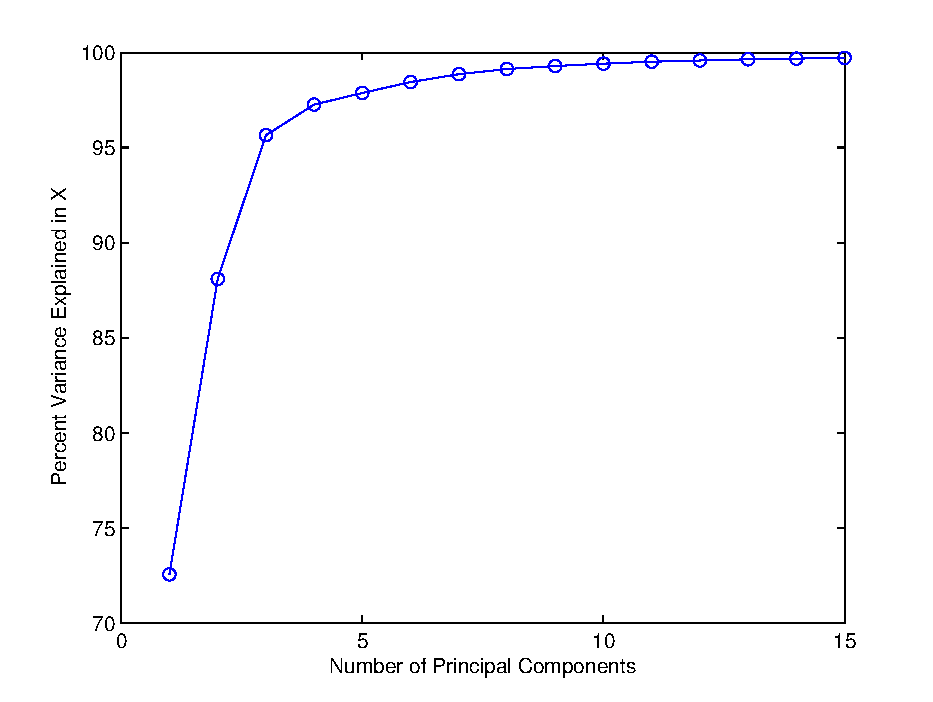
\includegraphics[width=.6\textwidth]{images/explain_PCR.pdf}\\
  \caption{The percent variance explained by the corresponding principal component}\label{pcrb1}
\end{figure}

We can see in the figure that when the number of principal components is greater than 3, the percent is greater than 95\%. It is really enough to keep the feature of the dataset using only 3 principal components.

And to find the smallest SMSE, we choose to use the grid search. The result of grid search is shown in Figure \ref{pcrb2}.
\begin{figure}[h]
  \centering
  % Requires \usepackage{graphicx}
  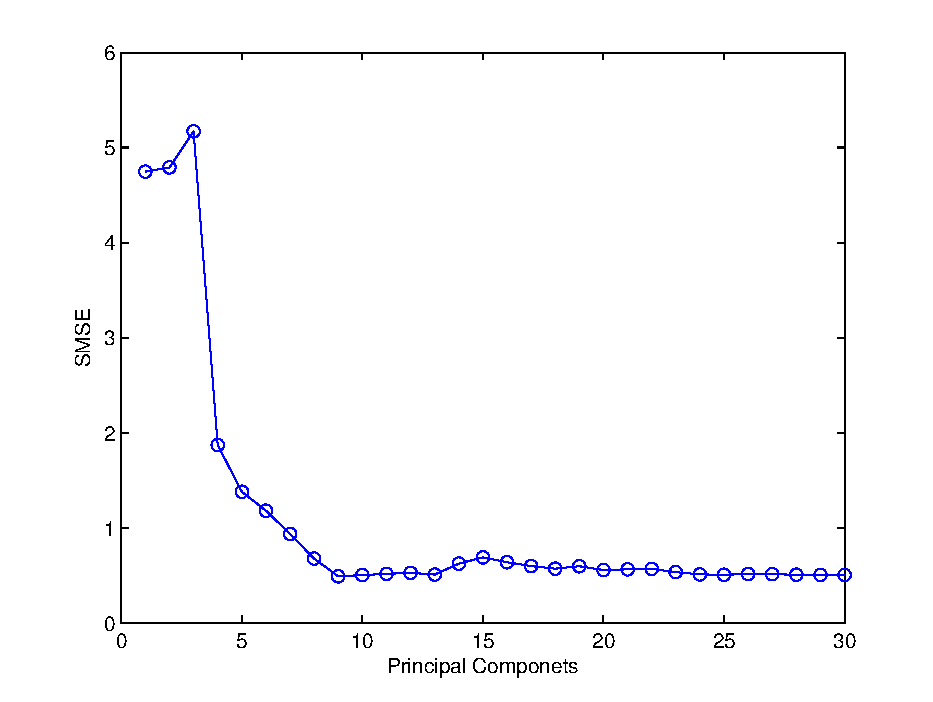
\includegraphics[width=.6\textwidth]{images/gsearch_PCR.pdf}\\
  \caption{The result of grid search}\label{pcrb2}
\end{figure}

\newpage
We can find that the SMSE is smallest when the number of principal components is equal to 9. The result predicted by PCR with 9 principal components is shown in Figure \ref{pic4}. And the SMSE is 0.098476.
\begin{figure}[h]
  \centering
  % Requires \usepackage{graphicx}
  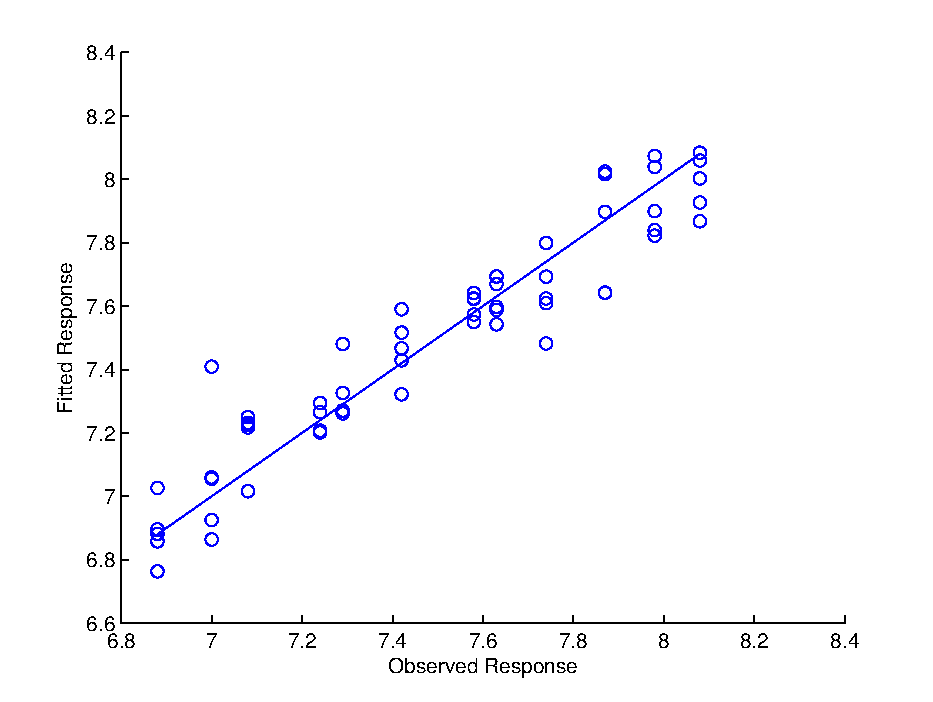
\includegraphics[width=.6\textwidth]{images/predict_PCR.pdf}\\
  \caption{PCR with 9 principal components}\label{pic4}
\end{figure}

The visualization of linear regression parameter $\bfv$ is shown in Figure \ref{pic5}.
\begin{figure}[h]
  \centering
  % Requires \usepackage{graphicx}
  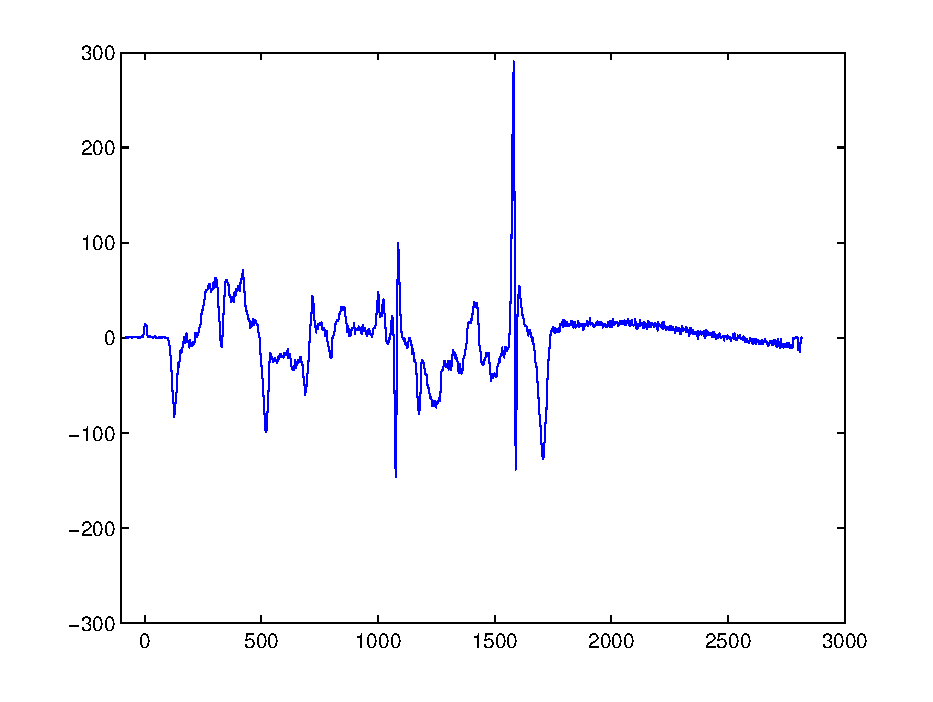
\includegraphics[width=.6\textwidth]{images/v_PCR.pdf}\\
  \caption{Plot of mean of $\bfv$ for PCR with 9 components}\label{pic5}
\end{figure}

\newpage
\subsection{Partial Least Squares Regression}
For PLSR, we also only consider the result on the data after normalization. 

It's the same with PLSR that the first problem needed to be solved is determining how many principal components should be used. We can also see the percent variance explained by the corresponding principal component in Figure \ref{plsrb1}.
\begin{figure}[h]
  \centering
  % Requires \usepackage{graphicx}
  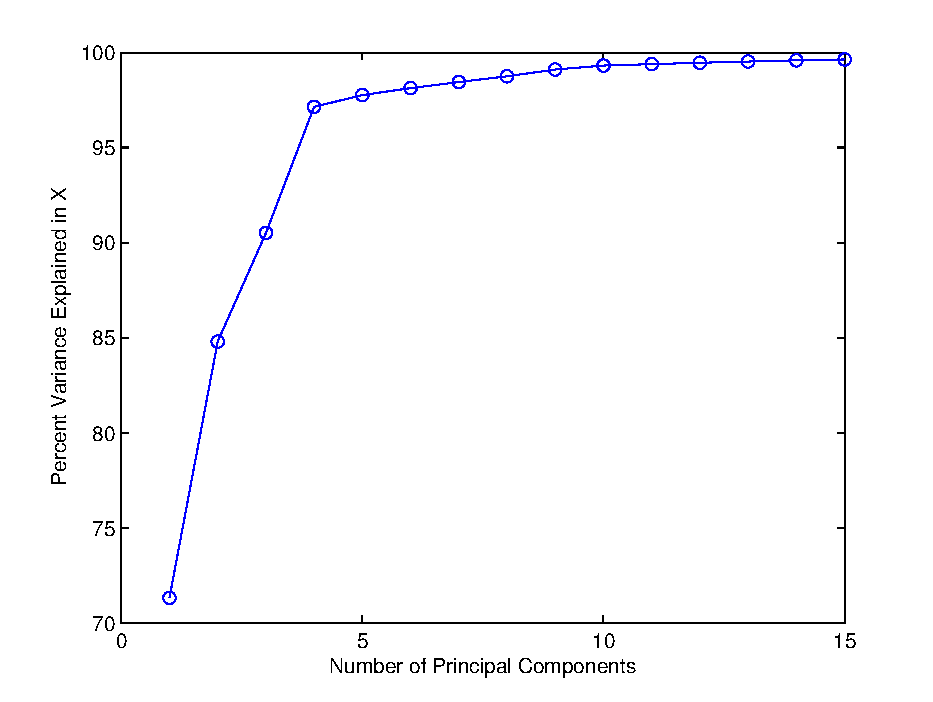
\includegraphics[width=.6\textwidth]{images/explain_PLSR.pdf}\\
  \caption{The percent variance explained by the corresponding principal component}\label{plsrb1}
\end{figure}

We can see in the figure that when the number of principal components is greater than 4, the percent is greater than 95\%. It is really enough to keep the feature of the dataset using only 4 principal components.

And we use the same method, grid search, to find the smallest SMSE. The result of grid search is shown in Figure \ref{plsrb2}.
\begin{figure}[h]
  \centering
  % Requires \usepackage{graphicx}
  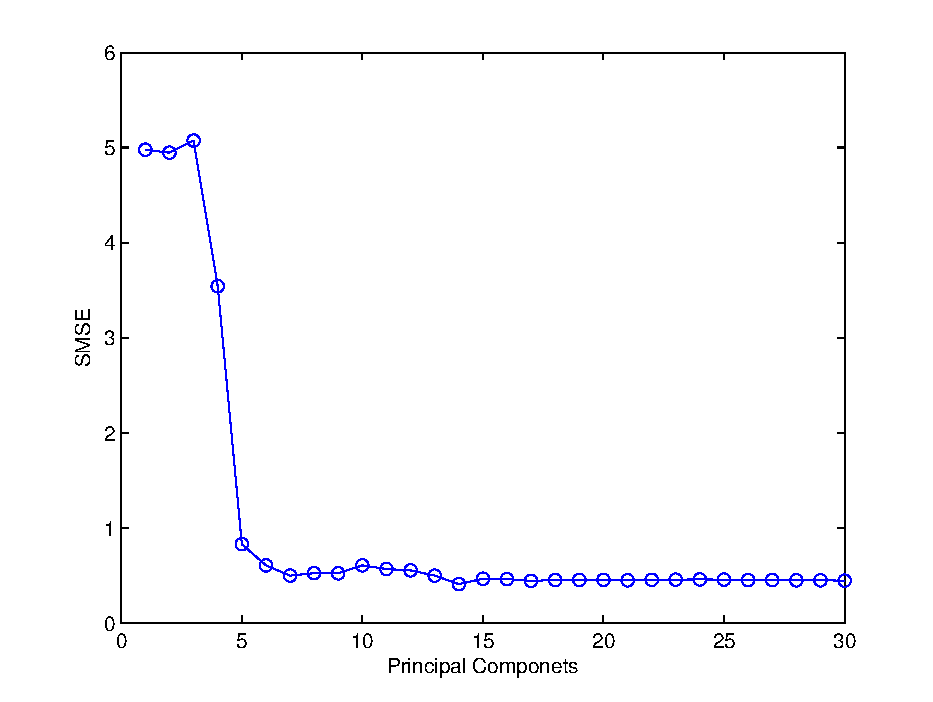
\includegraphics[width=.6\textwidth]{images/gsearch_PLSR.pdf}\\
  \caption{The result of grid search}\label{plsrb2}
\end{figure}

\newpage
We can find that the SMSE is smallest when the number of principal components is equal to 14. As we expected, this method has better performance than PCR, with SMSE 0.082091. 

The result predicted by PLSR is shown in Figure \ref{pic6}.
\begin{figure}[h]
  \centering
  % Requires \usepackage{graphicx}
  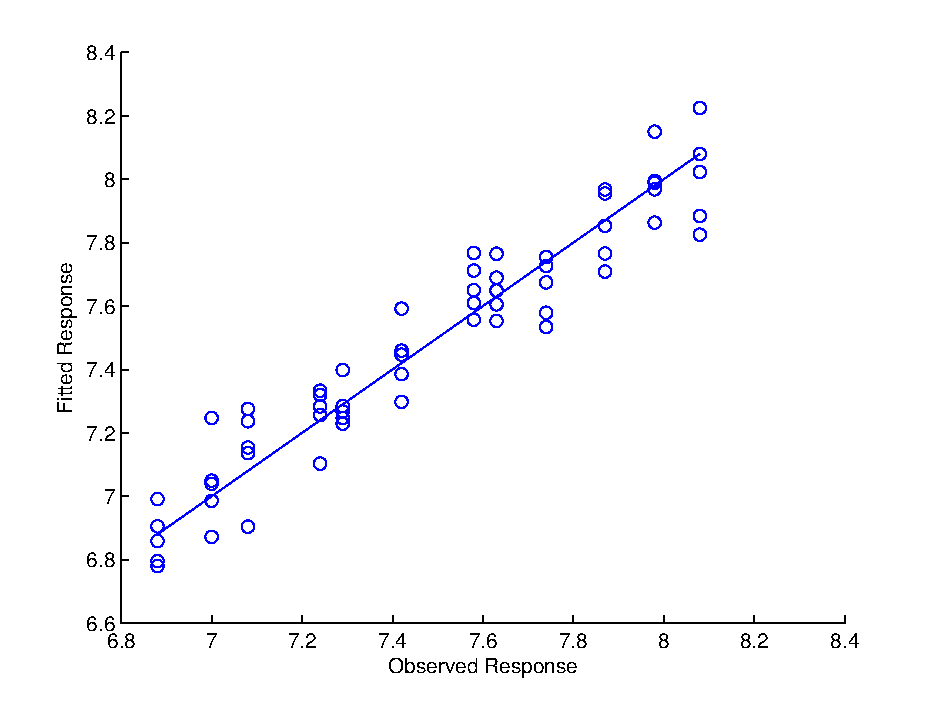
\includegraphics[width=.6\textwidth]{images/predict_PLSR.pdf}\\
  \caption{PLSR with 14 principal components}\label{pic6}
\end{figure}

The visualization of linear regression parameter $\bfv$ is shown in Figure \ref{pic7}.
\begin{figure}[h]
  \centering
  % Requires \usepackage{graphicx}
  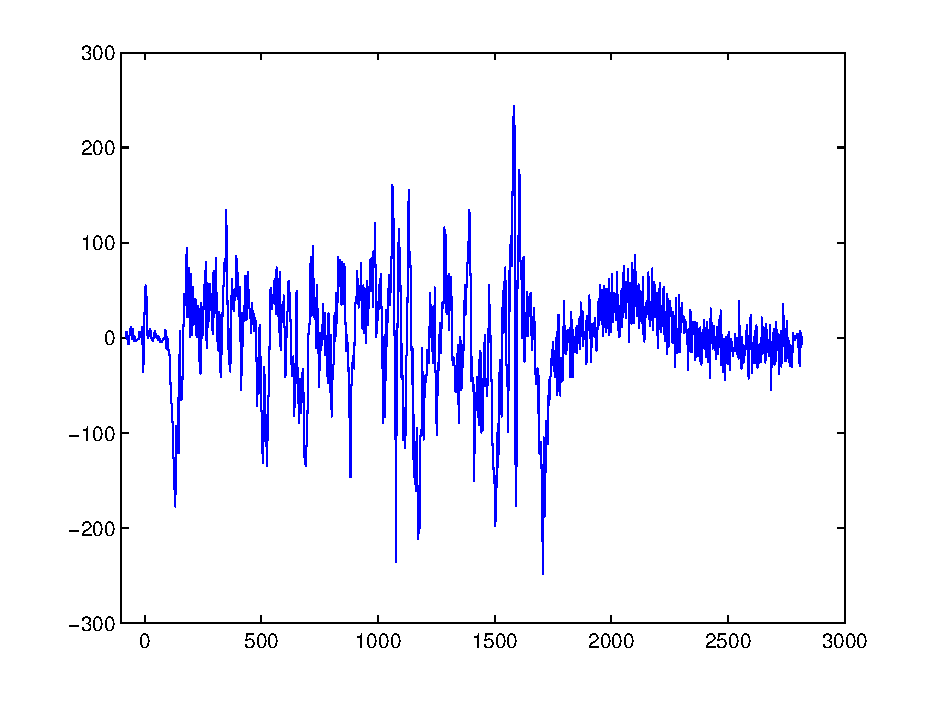
\includegraphics[width=.6\textwidth]{images/v_PLSR.pdf}\\
  \caption{Plot of mean of $\bfv$ for PLSR with 14 components}\label{pic7}
\end{figure}

As we can see, the curve is not that smooth like that of $\bfv$ for PCR and thus it's not easy for further analysis on it. So we try lasso regression in the next section to make the curve smoother. 

\subsection{Lasso Regression}
To make the curve smoother for further analysis and avoid the potential over-fitting problem, lasso regression is used to replace the linear regression in PCR and PLSR.
\begin{figure}[h]
  \centering
  % Requires \usepackage{graphicx}
  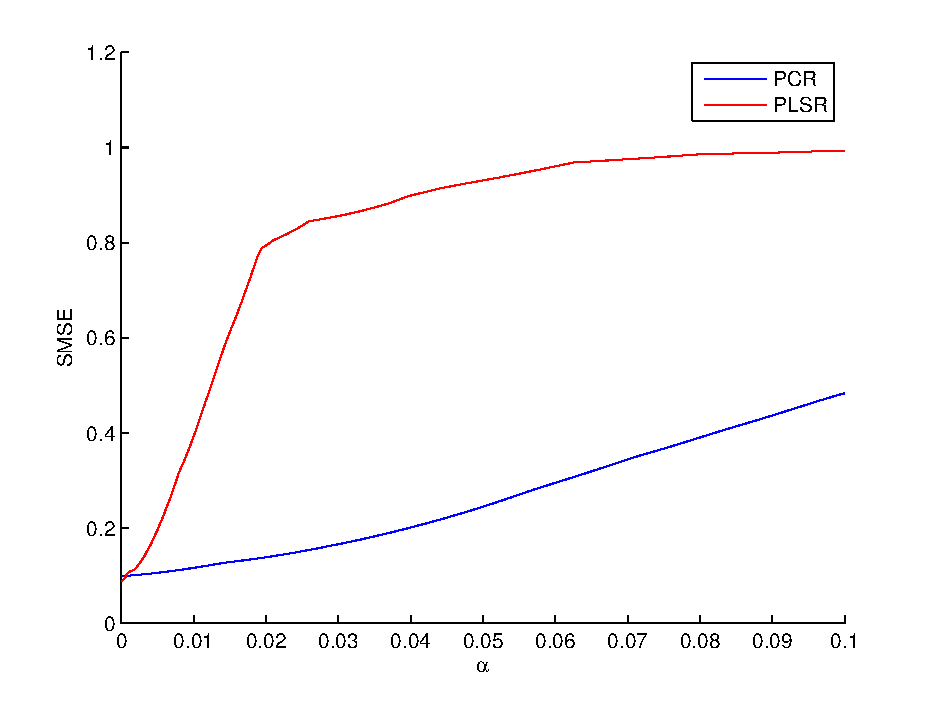
\includegraphics[width=.6\textwidth]{images/lasso.pdf}\\
  \caption{The relationship between SMSE and $\alpha$}\label{pic8}
\end{figure}

Figure \ref{pic8} shows the change of SMSE as the parameter $\alpha$ of lasso regression is increasing. 

As we can see in the figure, both the SMSE of PCR and PLSR are increasing. That means there are no over-fitting in the two regression methods before, and smoothing the curve of $\bfv$ is not a good way to improve the performance of those methods.

Moreover, we can find that the SMSE of PLSR increases much faster than that of PCR. As we know from the visualization of $\bfv$ shown before, the curve of $\bfv$ for PCR is much smoother than that of PLSR, so the $\alpha ||\bfv||$ part of the cost function may not affect the performance of PCR that much as $\alpha$ is increasing.
\subsection{Kernel Regression}
To find the best $\alpha$ in kernel regression, we also use grid search to determine which $\sigma$ should be chosen in Gaussian kernel.

Unfortunately, the performances are very poor no matter which $\sigma$ is chosen. When I try support vector regression with rbf kernel on the dataset, the performance is also very poor. The linear kernel, however, has a very good performance on this dataset. That may mean non-linear regression model  may not fit the data in this dataset.

\subsection{Gaussian Process Regression}
To use Gaussian process, we should determine two functions first, that is mean function and covariance function. And to do regression work, we should also determine which likelihood function is used. And inference method is also needed to find hyperparameters.

From the previous sections, we know that a linear mean function like
\begin{equation}
m(\bfx)=\sum_{i=1}^n a_ix_i + a_0
\end{equation}
is more suitable for our dataset, so this function is the only mean function we have chosen for later experiments.

As for covariance function, two functions have been chosen for experiments. The first one is squared exponential covariance function
\begin{equation}
k(\bfx_p,\bfx_q)=\sigma_0^2\exp\Big[-\frac{(\bfx_p-\bfx_q)'\times P^{-1} \times (\bfx_p-\bfx_q)}{2}\Big].
\end{equation}
Here, $P$ is equal to $\lambda$ times the unit matrix. And both $\sigma_0$ and $\lambda$ are hyperparameters. The second one is Matern covariance function
\begin{equation}
k(\bfx_p,\bfx_q)=\sigma_0^2\times f(\sqrt{d}r)\times \exp(-\sqrt{d}r).
\end{equation}
Here, $d$ is set to be 5 in our experiments, and function $f$ is set to be $f(t)=\frac{1+t+t^2}{3}$. And $r$ is the distance $\sqrt{(\bfx_p-\bfx_q)'\times P^{-1} \times (\bfx_p-\bfx_q)}$, while $P$ is the same matrix as above. So it's the same that both $\sigma_0$ and $\lambda$ are hyperparameters.

And since we're going to do regression work, we choose the traditional Gaussian function for likelihood function
\begin{equation}
f(x)=\frac{1}{\sigma\sqrt{2\pi}} \exp\Big[ -\frac{(x-\mu)^2}{2\sigma^2} \Big].
\end{equation}
Here, $\mu$ is the mean and $\sigma$ is the standard deviation. And only the standard deviation is in the hyperparameters.

And we have choose some different inference methods to get optimized hyperparameters. Table \ref{table1} shows the result for squared exponential covariance function, while Table \ref{table2} shows the result for Matern covariance function. Note that the two tables of results produced by experiments with the same mean function and likelihood function.

\begin{table}[h]
\centering
\begin{tabular}{|c|c|c|c|c|c|c|}
\hline
\textbf{No.} & GP01 & GP02 & GP03 & GP04 & GP05 & GP06 \\
\hline
\textbf{Method} & infExact & infEP & infLaplace & infVB & infKL & infLOO \\
\hline
\textbf{SMSE} & 0.085254 & 0.084868 & 0.085691 & 0.084877 & 0.085814 & 0.089122 \\
\hline
\end{tabular}
\caption{Result for squared exponential covariance function}\label{table1}
\end{table}
\begin{table}[h]
\centering
\begin{tabular}{|c|c|c|c|c|c|c|}
\hline
\textbf{No.} & GP07 & GP08 & GP09 & GP10 & GP11 & GP12 \\
\hline
\textbf{Method} & infExact & infEP & infLaplace & infVB & infKL & infLOO \\
\hline
\textbf{SMSE} & 0.086177 & 0.084075 & 0.083821 & 0.083809 & 0.084479 & 0.089021 \\
\hline
\end{tabular}
\caption{Result for Matern covariance function}\label{table2}
\end{table}

The result predicted by GP10 which has the best SMSE is shown in Figure \ref{pic9}.
\begin{figure}
  \centering
  % Requires \usepackage{graphicx}
  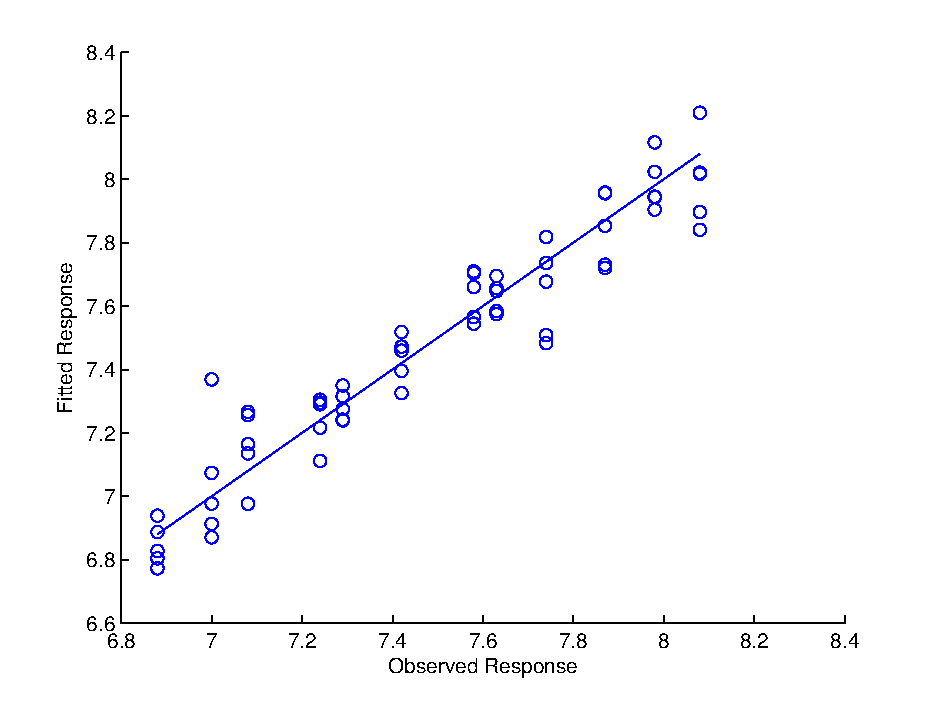
\includegraphics[width=.6\textwidth]{images/predict_GP09.pdf}\\
  \caption{Result of Gaussian process with the best SMSE}\label{pic9}
\end{figure}


\bibliography{report}\addcontentsline{toc}{section}{Reference}
\end{document}
